\documentclass[letterpaper]{article}

%% Language and font encodings
\usepackage[english]{babel}
\usepackage[utf8x]{inputenc}
\usepackage[T1]{fontenc}

%% Sets page size and margins
\usepackage[letterpaper,top=3cm,bottom=2cm,left=2cm,right=2cm,marginparwidth=1.75cm]{geometry}

%% Useful packages
\usepackage{amsmath}
\usepackage{graphicx}
\usepackage[colorinlistoftodos]{todonotes}
\usepackage[colorlinks=true, allcolors=blue]{hyperref}


\title{EE576 HW 2}
\author{Matt Ruffner}

\begin{document}
\maketitle

%%%%%%%%%%%%%%%%%%%%
%%%%%%%%%%%%%%%%%%%%
\section{}
First, frequency analysis in CrypTool 2.1 was run on the encrypted file to find the two most used encrypted letters: G and O. These two letters were then exored with the encoded equivalent of an 'E', the most common letter in the English language. The result of these two ex-ors were the letters 'C' and 'K'. Two descriptions were then preformed on the encrypted data until the result was coherent. The key used for success full decryption was 'KC'. The resulting decoded text is included in the attached file \texttt{q1decoded.txt}

\section{}
For this problem. The sample text included in \texttt{q2input.txt} was used. This was encoded with the Vigenere cipher three times, with the keys \textit{fox}, \textit{brownfox} and \textit{quickbrownfox}. The first two were able to be successfully decrypted with the Vigenere breaker component of CrypTool, however the third key produced was not able to be successfully decrypted. The input file was then decreased in length by a factor of two. The results indicated that a shorter amount of encrypted text offered less clues as to the correct encryption key. A second halving of the input text yielded  a wildly incorrect key that was also much shorter in length than previously.

\section{}
To decrypt the input file, \texttt{AES-ciphertext.bin}, JCryptTool was used, with no padding in Electronic CodeBlock mode. The result of the decryption is included in \texttt{q3output.txt}.

\section{}
The following tables depict the state bytes through one  round of the AES encryption process. The final \textit{MixColumns} step was calculated using the attached \texttt{mxmult.py} program.
\begin{table}[h!]
    \centering
    \parbox{5cm}{
        \centering
        \begin{tabular}{cccc}
            00 & 01 & 02 & 03 \\
            04 & 05 & 06 & 07 \\
            08 & 09 & 0A & 0A \\
            0C & 0D & 0E & 0F \\
        \end{tabular}
        \caption{Original Contents}
        \label{tab:mes1}
    }
    \parbox{5cm}{
        \centering
        \begin{tabular}{cccc}
            01 & 00 & 03 & 02 \\
            05 & 04 & 07 & 06 \\
            09 & 08 & 0B & 0B \\
            0D & 0C & 0F & 0E \\
        \end{tabular}
        \caption{After AddRoundKey}
        \label{tab:mes2}
    }
    \parbox{5cm}{
        \centering
        \begin{tabular}{cccc}
            7C & 63 & 7B & 77 \\
            6B & F2 & C5 & 6F \\
            01 & 30 & 2B & 2B \\
            D7 & FE & 76 & AB \\
        \end{tabular}
        \caption{After SubBytes}
        \label{tab:mes3}
    }
\end{table}


\begin{table}[h!]
    \centering
    \parbox{5cm}{
        \begin{tabular}{cccc}
            7C & 6B & 01 & D7 \\
            F2 & 30 & FE & 63 \\
            2B & 76 & 7B & C5 \\
            AB & 77 & 6F & 2B \\
        \end{tabular}
        \caption{After ShiftRows}
        \label{tab:mes4}
    }
    \parbox{5cm}{
        \centering
        \begin{tabular}{cccc}
            AE & 47 & EC & 69 \\
            B2 & 1E & E3 & 75 \\
            D9 & D2 & 44 & BF \\
            FB & E9 & 58 & 75 \\
        \end{tabular}
        \caption{After MixColumns}
        \label{tab:mes5}
    }
\end{table}




\section{}
The unmodified image is shown in Fig. \ref{fig:apple}. The image encrypted with AES in ECB mode is shown in Fig. \ref{fig:appleecb}. The image encoded with AES in CBC mode is shown in Fig. \ref{fig:applecbc}.

\begin{figure}[h!]
    \centering
    \begin{minipage}{5cm}
        
\includegraphics[width=5cm]{apple.png}
        \caption{\texttt{apple.bmp}}
        \label{fig:apple}
    \end{minipage}
    \hspace{0.7cm}
    \begin{minipage}{5cm}
        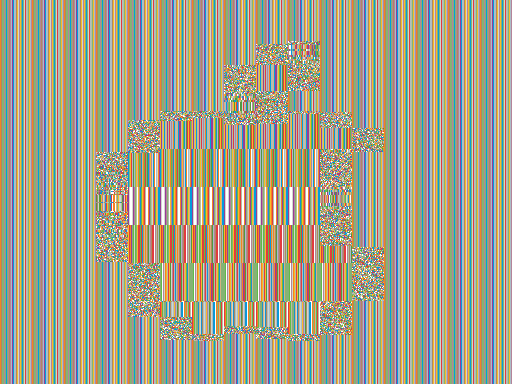
\includegraphics[width=5cm]{appleecb.png}
        \caption{\texttt{appleecb.bmp}}
        \label{fig:appleecb}
    \end{minipage}
    \hspace{0.7cm}
    \begin{minipage}{5cm}
        
\includegraphics[width=5cm]{applecbc.png}
        \caption{\texttt{applecbc.bmp}}
        \label{fig:applecbc}
    \end{minipage}
    \hfill
\end{figure}


\section{}
\paragraph{1}
  We know the random vector, \textit{v}, since it is always the first 80 bits. With the addition of this  information, all of $v$, $c$, and $k$ are known. Thus, the the message can be decrypted by computing RC4$(v||k) \oplus c$.

\paragraph{2}
  By observing the random vector $v$ across transmissions. The same $v$ implies the same key stream was used to encrypt the messages.

\paragraph{3}
  The key stream varies with random 80 bit $v$ since the key is fixed. Brute-force collision search is $O(2^{n/2})$, where $n$ is the number of bits. Thus, after $2^40$ transmissions the random $v$ will probably be repeated.

\paragraph{4} 
  This implies that the key should be changed before $2^{40}$ transmissions have occured.

\section*{Acknowledgements}
This homework was completed in collaboration with Jordan Caudill.


\end{document}